\section{Limb Circumference}

Limb circumference uses point cloud partitioning combined with the plane pulling algorithms associated with volume estimation that allow for the convex hull of planes in the respective area of the point cloud to be calculated and an approximate circumference returned.

\subsection{Partitioning the Point Cloud}

Partitioning of the point cloud so that planes could be taken for circumference calculation required translation of the inferred skeleton points tracked by the Kinect into Point Cloud space so that the appropriate bounds around each cross section of the point cloud could be taken. These bounds were defined for each of the respective feature points for limbs of interest. The encapsulation of the captured scan in the \texttt{PointCloud} data structure allowed a region of the point cloud to be extracted using the \texttt{range} function which took an (x,y,z) interval defined in point cloud space from the uniquely indexed underlying KD-Tree structure. A check was implemented when extracting the point cloud to ensure that sub regions were actually being extracted from the correct region. If the bounds were non-sensical (\textt{$x_{min} > x_{max}$}, for example) then the skeleton had not been tracked properly (as was often the case when it had inferred particular body parts during the scan incorrectly or had tracked an object that resembled a skeleton. The user was then asked to rescan to ensure an accurate capture. \\

The partitioning of the point cloud was fixed to the following local areas of the body; \emph{chest, shoulders, left arm, right arm, left leg, right leg, waist}. Any further partitioning of these limbs would have resulted in varied point clouds depending on the subject and high degree of noise from the increasing degradation in depth point quality at these levels.\\

\subsection{Corrective Constants}

\begin{figure}
\begin{center}
    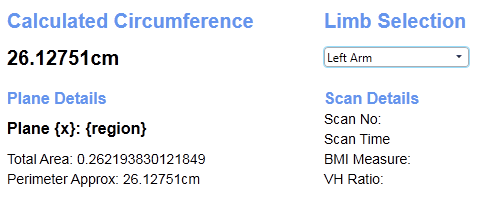
\includegraphics[scale=0.6]{zscreenshots/limbdetails.png}
    \caption{Detailed view of limb circumference for the left arm of the Papaconstantinou subject}
\end{center}
\end{figure}


The requirement for corrective constants for the limb circumference measurement is as a result of the quality of the point clouds partitioned. The quality of the partitioned point clouds is dependent on the accuracy of the skeletal points that have been translated into point cloud space, if this translation is inaccurate than the partition will be poor or incorrect. Even if the quality of the point cloud partitioned well, the presence of clothes, the quality of the point cloud's affine ICP and the size of the patient all attribute to the need for correction to the calculated circumferences. In particular, while the mapping between the skeletal points and the point cloud is relatively accurate; for patients of an above average nature, it may be possible that the bounds specified do not fully capture the limb and thus underestimate the total circumference of a particular area of the body. These corrective constants are determined fully on a number of patients in the \emph{Testing} section of this report.
